\documentclass[12pt]{article}
\usepackage{graphicx}
%\usepackage{showframe}
\usepackage[top=1.0in, bottom=1.0in, left=1.5in, right=1.0in]{geometry}
\title{A Modern Version Of Space Invaders}
\author{Rian Fitzgerald}
\parindent 0ex
\setlength{\parskip}{1em}
\begin{document}
\pagenumbering{gobble}
%\maketitle
\newpage
\begin{center}
\section*{}
	
\includegraphics[scale=1]{uni-limerick-crest.png}
	
	{\Large Department of Computer Science and Information Systems
	
	Title: A modern version of Space Invaders
	
	By: Rian Fitzgerald 13121626
	
	Course: Computer Games Development LM110
	
	Supervisor: Annette McElligott}
	
\end{center}
\newpage
\pagenumbering{roman}
\begin{center}
\section*{Project Summary}
\end{center}
This project is an advanced version of the classic game Space Invaders. It will retain some of the core mechanics and add some features that will provide a challenge for the player. 

There are two parts to this project, the game and the supporting website. The website is used to create accounts for players as well as having a leader board which displays data about the player (for example, their high score, time played and highest level achieved). 

This project uses the same perspective as the original game (top down, two dimensional). The difference between this version and the original is that it will become harder to beat as the players score increases. The objective of the game is to survive as long as possible and achieving the highest score possible. 

This project will use modern tools and techniques as this was a limiting factor in the original implementation. These factors are discussed in more detail in the Background and Research portion of this report. 

\newpage
\begin{center}
\section*{Acknowledgments}
\end{center}
I would like to acknowledge my family and friends for providing guidance and support for me during my years at college. 
\newpage
\begin{center}
\section*{Declaration}
\end{center}
\newpage

\begin{center}
\tableofcontents
\end{center}

\newpage
\pagenumbering{arabic}



\begin{center}
\section{Introduction}
\end{center}

\begin{center}
\subsection{General Introduction} 
\end{center}
This chapter will give a brief description of the chapters that follow. Chapter two  discusses that background and research that went into this project. Chapter three will show case some of the design that went into this project. Chapter four will address some of the implementation and issues encountered. Chapter five will showcase the testing and evaluation used in the project. The final chapter discusses the conclusions and possible further development of this project.

\begin{center}
\subsection{Motivating Factors}
\end{center}
The main motivation for undertaking this project was to improve the Space Invaders game. From the research completed (this is discussed in Chapter 3), many clones have a set difficulty. This results in an imbalance in the difficulty. A highly skilled player will be able to get a higher score quite easily. The result of this project has created a game that uses information collected by the player to make it more difficult for them to beat. 

A secondary motivation to complete this project was to become familiar with using a modern game engine. It would be a useful skill to add to my repertoire, especially if I want to apply for a job in a game company after college. 

Another motivation for doing this project is to increase my knowledge in web based technologies. As most companies have a web presence it would be useful to know about web technologies, especially those based around JavaScript. 

The final motivation for completing this project is to combine the knowledge I have learned from various modules. This project incorporates aspects of Programming, Object Orientated Programming, Database Systems, Distributed Systems and Systems Analysis and Design. Principles learned from these modules will be applied in the project

\begin{center}
\subsection{Objectives of Proposed Work}
\end{center}
This project has two main objectives with multiple elements to be completed. The two primary objectives are the game and the website. 

The following list details the objectives to be completed for the game.

\begin{enumerate}
\item Programming the initial game using simple graphics.
\item Refining the game mechanics.
\item Program a login screen for the game to allow a player to login so their details can
be recorded.
\end{enumerate}

The next list details the objectives to be completed for the website.

\begin{enumerate}
\item Programming the website.
\item Programming the server.
\item Responding to any GET, POST, PUT and DELETE commands to make the
website RESTful.
\item Creating the database and populate it with test data.
\item Use a testing framework to test if the correct data is being transferred to the
various parts of the project.
\end{enumerate}
\newpage

\begin{center}
\section{Background and Research}
\end{center}
The background and research section discusses the previous implementations of Space Invaders and the considerations that the original designer had to consider. It will also analyse the technologies that will power this project. 

\begin{center}
\subsection{Analysis of Existing Products}
\end{center}
The original Space Invaders was very primitive in its implementation. It was so primitive that it was unable to render many colours and had to rely on a colour overlay. (arcade-museum.com, 2016). The specification for some of the system is given below


\begin{itemize}
	\item Processor: Intel 8080
	\item Raster graphics on a CRT monitor
	\item Texas Instruments SN76477
\end{itemize}

An interesting point to note is that the graphics were drawn using the processor. This was due to the lack of dedicated graphics processing units at the time. It also explains why the graphics were primitive by today's standards (for example, pixel based with little colouring).

In 1980 a version of Space Invaders was ported to the Atari 2600 (gamespy.com, 2016). This had a number of advantages over the original. The biggest advantage was that the colour palette was increased. Other hardware improvements included the addition of RAM and cartridges that could have memory included. (problemkaputt.de/, 2016)

At the time of writing this report, there are many clones that exist. These clones are available on many platforms from the original game to iOS (kotaku.com, 2016). These clones can differ in many ways from the original. Some will have different aesthetics while others will have different mechanics. The table below is a compiled list of some of the data available about space invaders clones (bandainamcoent.eu, gamespy.com, ign.com, kotaku.com, theisozone.com, 2017).

\begin{center}
    \begin{tabular}{ | p{2.25cm} | p{2.5cm} | p{4.5cm} | p{4cm} |} \hline
    Name & Platform(s) & Released & Features \\ \hline
    Space Invaders (Original) & Arcade, Atari 2600, Nintendo Entertainment System, iOS & 1978, 1980, 1985, 2009 & Raster graphics \\ \hline
    
    Space Invaders Part II, Space Invaders Deluxe (USA) & Arcade, Game Boy & 1979, 1990 & Gameboy version allowed multiplayer, USA version had updated graphics\\ \hline
    
    Space Invaders '95 & Arcade & 1995 & Updated graphics  \\ \hline
    
	Space Invaders 1999, Space Invaders X (Japan) & Playstation, PC, Nintendo 64, Game Boy Color & 1999 & 2D and 3D graphics, competitive mode, cooperative mode,   \\ \hline 
	
	Space Invaders Evolution, Space Invaders: Galaxy Beat (Japan) & Playstation Portable & 2005 & Updated graphics, sounds and gameplay, multiplayer mode, rhythm action gameplay \\ \hline
	
	Space Invaders Extreme & Nintendo DS, Playstation Portable, Xbox 360 & 2008, 2009 & Integrated musical elements \\ \hline
	
	Space Invaders Infinity Gene & iOS, Playstation 3, Xbox 360, Android & 2009, 2010, 2013 & Updated graphics\\ \hline
    \end{tabular}
\end{center}

\newpage
\begin{center}
\subsection{Unity Game Engine}
\end{center}
The Unity engine is a multiplatform game engine. It allows developers to target a range of devices for example PC, Android, iOS and Xbox, to name a few. It uses one click deployment to build solutions for as many devices that are required. (https://unity3d.com/, 2016).

The engine supports a multitude of file formats for images, audio, video and text. The engine abstracts the more difficult aspects of creating a game such as optimisation and graphics rendering. For graphics, it targets APIs depending on which system is selected for the build. Windows can use both Direct3D and OpenGL, Android and iOS use OpenGL ES and consoles use proprietary APIs.

Programming in Unity can be achieved by using a number of languages. The most widely used language for Unity is C sharp. JavaScript can also be used; however, it is not the same JavaScript that is used for web browsers. It is commonly referred to as UnityScript. (answers.unity3d.com/, 2016). A third language called Boo is also available, however it is now deprecated. It is not documented by Unity anymore, although it will still compile. (forum.unity3d.com, 2016).

Due to its better support and documentation, C sharp will be the language used to implement the game portion of this project.


\begin{center}
\subsection{Unreal Engine}
\end{center}
Another popular choice for developing games is Unreal Engine. It is one of the biggest competitors to Unity. It is also a multiplatform game engine and can export builds for a range of devices such as PC, Mac, Linux, XBOX and Playstation, to name a few. (https://www.unrealengine.com).

As with Unity, Unreal Engine supports many file formats. It also enables developers to accomplish more as the more difficult parts of game programming is abstracted. Programming in Unreal is achieved using two methods. The first is using C++ and utilising the Unreal API. The second method uses blueprints. Blueprints in Unreal are a style of visual coding where the developer drags, drops and connects nodes to get the desired functionality. However these blueprints are not as good performance wise when compared to C++. (https://forums.unrealengine.com.) 

\begin{center}
\subsection{MongoDB}
\end{center}
MongoDB is a high performance, scalable, document orientated NoSQL database solution. (stackoverflow.com, 2017). MongoDB uses a JSON-like document with schemas. JSON is a lightweight data format that is easy for humans to read and write as well as to parse for machines. Figure 3.1 shows an example of some data in the JSON format.

JSON is built upon two structures: 
\begin{itemize}
	\item A collection of key/value pairs that correspoind to an abject, record, dictionary, hash table, keyed list or an associative array, depending on which language is being used.
	\item A list of ordered values that correspond to an array, vector or similar data structure. 
\end{itemize}

(json.org, 2017)

\begin{center}
	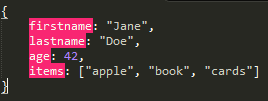
\includegraphics[scale=1]{json_no_id.PNG}
	
	\caption Figure 3.1: Data in JSON format
\end{center}

Because MongoDB is a NoSQL solution the schema is not enforced as strictly as it would in a relational database. The dynamic schema means that each document can have different key/value pairs and can still be inserted into the database. The table shown below summarises the differences between a Relational Database Management System (for example, MySQL) and MongoDB.

\begin{center}
    \begin{tabular}{| l | l |}
    \hline
    Relational Database Management System & MongoDB  \\ \hline
    Table & Collection \\ \hline
    Tuple or Row & Document \\ \hline
    Column & Field \\ \hline
    Primary Key & Key id provided by MongoDB \\ \hline
    \end{tabular}
\end{center}

The {\_}id provided by MongoDB is a 12 byte hexadecimal number which ensures the uniqueness of every document. This hexadecimal number is construced as follows:

\begin{itemize}
	\item The first 4 bytes are a timestamp since the ObjectId's creation. This uses the seconds elapsed since the Unix epoch.
	\item The next three bytes are a machine identifier.
	\item The following 2 bytres are a process ID
	\item The final 3 bytes are a counter that starts at a random value
\end{itemize}

If a document does not specify a unique {\_}id field, MongoDB will generate an ObjectId for this field. This is because the {\_}id is used as a primary key (docs.mongodb.com, 2016). Figure 3.2 shows the same data as Figure 3.1 but now includes an the {\_}id field. 

\begin{center}
	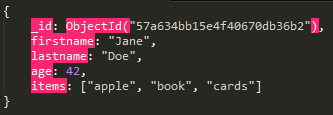
\includegraphics[scale=1]{json_id.PNG}
	
	\caption Figure 3.2: Data including the 12 byte hexadecimal {\_}id field. In this example the {\_}id was automatically generated from MongoDB. 
\end{center}

\begin{center}
\subsection{MySQL}
\end{center}
MySQL is a free open source Relational Database Management System (RDMS) that uses Structured Query Language (SQL) to perform database operations. Unlike MongoDB, MySQL must follow a schema. A schema is a logical group of tables, procedures and views that relate to one type of object (for example an employee schema). (stackoverflow.com, 2017)

MySQL is also fully ACID compliant. ACID stands for: 
\begin{itemize}
	\item Atomic: an update to a document with fully completes or doesn't
	\item Consistent: no parital update will be read
	\item Isolated: no dirty update will be read
	\item Durable: 
\end{itemize}

MongoDB is not as ACID compliant as MySQL. It is compliant at the document level. What MongoDB lacks is transactions. This is the ability to revert any updates to multiple documents. (stackoverflow.com, 2017).

Unlike MongoDB, when using MySQL the developer must decide on a primary key to use. This can be any value the developer chooses but a good practice is to use a type of user identifier that is automatically incremented when a new user is entered. The syntax for this statement might look like the following: 

\begin{verbatim}
CREATE TABLE IF NOT EXISTS Users(
	userID INT UNSIGNED NOT NULL AUTO_INCREMENT,
	PRIMARY KEY(userID)
);
\end{verbatim}

\end{list}   

\begin{center}
\subsection{ExpressJS}
\end{center}
ExpressJS is a flexible JavaScript web application framework which uses NodeJS to create features for web and mobile applications (expressjs.com, 2017).

It is minimal and provides tools to build applications, with many more plugins available via the Node Package Manager (npm). ExpressJS is similar to Rails for Ruby and Django for Python. Unlike Ruby on Rails or Django there is no documented best way to use the ExpressJS framework. Because it is written in JavaScript and uses NodeJS, express is able to interact with MongoDB in order to retrieve, insert, update and remove documents from a database.

\begin{center}
\subsection{AngularJS}
\end{center}
AngularJS is a client-side JavaScript framework that is developed by Google. HTML is useful for declaring static views but fails when trying to declare a dynamic view. Other frameworks deal with this issue by abstracting technologies to manipulate the Document Object Model (DOM). These solutions don’t address the root problem which is HTML (angularjs.org/, 2017). AngularJS addresses this issue by extending HTML which is achieved by using directives and binds data to HTML using expressions.

AngularJS is used to develop the frontend elements of a system. Angular uses the Model View Controller (MVC) pattern in order to separate the representations of the data from how it is displayed to the user. Because it is JavaScript based, AngularJS is able to communicate with the other chosen technologies easily.

\begin{center}
\subsection{NodeJS}
\end{center}
NodeJS is a server side solution for JavaScript. It is comparable to an Apache webserver for PHP. It is not a JavaScript framework but many of the modules it uses are written in JavaScript. It is built upon Google Cromes V8 JavaScript engine. NodeJS uses an event driven, non-blocking I/O model the makes it lightweight and efficient (nodejs.org/en/, 2017).

A non-blocking I/O (also known as an asynchronous I/O) means that an I/O request will be queued straight away and the function returns. The I/O is processed at a later point. A blocking I/O thread cannot process anything else until the I/O is complete. In the case of sockets, this could result in a long waiting time. NodeJS uses only uses one thread to service all requests. (stackoverflow.com/, 2017)

The advantage of using NodeJS is that it has its own package manager, similar to Ubuntu, called Node Package Manager (npm for short). This allows developers to share libraries of code as well as managing versions of the code. This is how the ExpressJS framework will be integrated into the project.

\begin{center}
	\subsection{Apache Server}
\end{center}
The Apache web server is a software product which aims to create a feature rich, robust, commercial grade, open source HTTP server. (httpd.apache.org, 2017). 

The features which Apache supports are implemented in compiled modules which can range from server programming to authentication schemes. It is often used with MySQL and PHP to crate web applications.

Apache allows developers to control access to different web pages by using different modules that are provided, however it does not give as much control as a NodeJS server. Apache does allow developers to create their own modules however it is not as simple as using NodeJS.

\begin{center}
	\subsection{Research Conclusions}
\end{center}
From the research completed of the existing games, it is clear that many existing implementations don't address the fact that the difficulty stays the same for the game. The original Space Invaders did have a feature where the enemies would get faster the less there were, however this was a bug that the developer made a mechanic out of. Some solutions to address this problem include creating a template that uses the existing players data to instantiate a level based on this data. Another solution would be to change properties of the enemy as the game goes on. 

The Unity game engine will be used to implement the functionality of the game . This decision is based on some of the pitfalls of Unreal engine. Although Unreal engine is a more commonly used solution, it didn't suit this project. This is because the blueprints technology used is too simplified and C++ can be over complicated. Unity is a happy medium between these as it uses the C{\#} language for functionality. This also gives the advantage of accessing the .NET framework if necessary. 

For the web application portion of this project, MongoDB, ExpressJS, AngularJS and NodeJS technologies will be used. This decision was based on a number of factors. Firstly is previous experience using these technologies. Secondly is the fact that all these technologies are JavaScript based and MongoDB uses JSON which enables data to be easily passed to and from the server. This is in contrast to using Apache, MySQL and PHP which use different technologies that allow the same functionality. The final factor influencing this decision is that JavaScript technologies are becoming more popular and further experience using these would be beneficial in a future career. 

\newpage
\begin{center}
\section{Design}
\end{center}
The design portion of this report will deal with the various thought processes behind the design of the many parts in this project. 

\begin{center}
\subsection{Game Design}
\end{center}

\begin{center}
\subsection{Database Design}
\end{center}

\begin{center}
\subsection{Website Design}
\end{center}

\begin{center}
\section{Implementation}
\end{center}

\begin{center}
\section{Testing and Evaluation}
\end{center}

\begin{center}
\section{Conclusions and Further Development}
\end{center}

\begin{center}
\section{Appendicies}
\end{center}

\begin{center}
\section{References}
\end{center}
Angularjs.org (2017) \textit{ngController} [online], available: https://docs.angularjs.org/api/
\hangindent=0.5in ng/directive/ngController [accessed 1 January 2017]

Apache (2017) \textit{What is the Apache HTTP Server Project?} [online], available: https://httpd.apache.org/ABOUT_APACHE.html#What [accessed 6 April 2017]

Atari 2600 Specifications (2016) \textit{Technical Data} [online], available: http://problemka
\hangindent=0.5in putt.de/2k6specs.htm [accessed 29 December 2016]

Bandai Namco \textit{Space Invaders Evolution} [online], available:
https://www.bandainamc
\hangindent=0.5inoent.eu/product/space-invaders-evolution/psp [accessed
4 January 2017]

Express (2017) \textit{Web Application} [online], available: http://expressjs.com/ [accessed 
\hangindent=0.5in 1 January 2017]

Gamespy (2016) \textit{The Gamespy Hall of Fame} [online], available: https://web.archive.
\hangindent=0.5in org/web/20080408152913/http://archive.gamespy.com/legacy/halloffame/spa
\hangindent=0.5inceinvaders.shtm [accessed 30 December 2016]

IGN (2008) \textit{Space Invaders Extreme} [online], available: http://ie.ign.com/games/space-
\hangindent=0.5in invaders-extreme/nds-965078 [accessed 4 January 2017]

JSON (2017) \textit{Introducing JSON ECMA-404 The JSON Data Interchange Standard} [online], available: \hangindent=0.5in http://www.json.org/ [accessed 1 January 2017]

Kotaku (2016) \textit{Space Invaders Infinity Gene Micro-Review: Evolve or Die} [online], 
\hangindent=0.5in available: http://kotaku.com/5328750/space-invaders-infinity-gene-micro-rev
\hangindent=0.5in iew-evolve-or-die [accessed 30 December 2016]

MongoDB (2017) \textit{BSON Types} [online], available: https://docs.mongodb.com/manua
\hangindent=0.5in l/reference/bson-types/#objectid [accessed 1 January 2017]

NodeJS (2017) \texit{Home} [online], available: https://nodejs.org/en/ [accessed 2 January 
\hangindent=0.5in 2017]

Stack Overflow (2009) \textit{What good are SQL Server schemas?}, [online] available: http://stackoverflow.com/questions/529142/what-good-are-sql-server-schemas [accessed 5 April 2017]

Stack Overflow (2017) \textit{MongoDB} [online], available:
http://stackoverflow.com/questio
\hangindent=0.5in ns/tagged/mongodb [accessed 1 January 2017]

Stack Overflow (2011) \textit{What does MongoDB not being ACID compliant really mean?} [online], available: http://stackoverflow.com/questions/7149890/what-does-mongodb-not-being-acid-compliant-really-mean [accessed 5 April 2017]

Stack Overflow (2013) \textit{What is non-blocking or asynchronous I/O in Node.js?} [on
\hangindent=0.5in line], available: http://stackoverflow.com/questions/10570246/what-is-non-bl 
\hangindent=0.5inocking-or-asynchronous-i-o-in-node-js [accessed 2 January 2017]

The International Arcade Museum (2016) \textit{Space Invaders} [online], available: http://w
\hangindent=0.5in ww.arcade-museum.com/game{\_}detail.php?game{\_}id=9662 [accessed 29 December 2016]

The ISO Zone (2015) \textit{Space Invaders} [online], available:
http://www.theisozone.com/
\hangindent=0.5in downloads/pc/windows-games/space-invaders-12/
[accessed 4 January 2017]

Unity (2016) \textit{Build once, deploy anywhere} [online], available: https://unity3d.com/un
\hangindent=0.5in ity/multiplatform [accessed 30 December 2016]

Unity (2009) \textit{How should I decide if I should use C#, JavaScript (UnityScript) or 
\hangindent=0.5in Boo for my project?} [online], available: http://answers.unity3d.com/questions/75
\hangindent=0.5in 28/how-should-i-decide-if-i-should-use-c-javascript-u.html [accessed 30 December 2016]

Unity (2015) \textit{Will Boo ever come back?} [online], available:
https://forum.unity3d.com
\hangindent=0.5in m/threads/will-boo-ever-come-back.375988/ [accessed 30
December 2016]

Unreal (2014) \textit{[Twitch] Fortnite Developers Discussion - Apr. 17, 2014} [online], \hangindent=0.5in available: https://forums.unrealengine.com/showthread.php?3035-New-Twitch-\hangindent=0.5in -with-Fortnite-developers-Thursday-April-17&p=19464&viewfull=1#post19464 [accessed 05 April 2017]

Unreal (2017) \textit{What is Unreal Engine 4} [online], available: https://www.unrealengine.com\hangindent=0.5in /what-is-unreal-engine-4 [accessed 5 April 2017]

\newpage
\begin{center}
\section{Bibliography}
\end{center}

%\begin{center}
%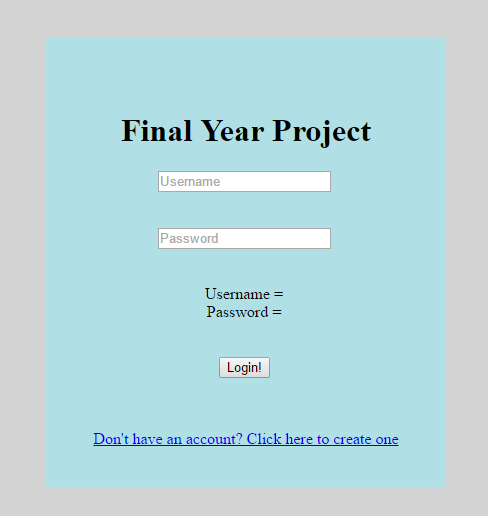
\includegraphics[scale=0.5]{photo.png}
%\end{center}


\end{document}